\documentclass{article}\usepackage[]{graphicx}\usepackage[]{xcolor}
% maxwidth is the original width if it is less than linewidth
% otherwise use linewidth (to make sure the graphics do not exceed the margin)
\makeatletter
\def\maxwidth{ %
  \ifdim\Gin@nat@width>\linewidth
    \linewidth
  \else
    \Gin@nat@width
  \fi
}
\makeatother

\definecolor{fgcolor}{rgb}{0.345, 0.345, 0.345}
\newcommand{\hlnum}[1]{\textcolor[rgb]{0.686,0.059,0.569}{#1}}%
\newcommand{\hlsng}[1]{\textcolor[rgb]{0.192,0.494,0.8}{#1}}%
\newcommand{\hlcom}[1]{\textcolor[rgb]{0.678,0.584,0.686}{\textit{#1}}}%
\newcommand{\hlopt}[1]{\textcolor[rgb]{0,0,0}{#1}}%
\newcommand{\hldef}[1]{\textcolor[rgb]{0.345,0.345,0.345}{#1}}%
\newcommand{\hlkwa}[1]{\textcolor[rgb]{0.161,0.373,0.58}{\textbf{#1}}}%
\newcommand{\hlkwb}[1]{\textcolor[rgb]{0.69,0.353,0.396}{#1}}%
\newcommand{\hlkwc}[1]{\textcolor[rgb]{0.333,0.667,0.333}{#1}}%
\newcommand{\hlkwd}[1]{\textcolor[rgb]{0.737,0.353,0.396}{\textbf{#1}}}%
\let\hlipl\hlkwb

\usepackage{framed}
\makeatletter
\newenvironment{kframe}{%
 \def\at@end@of@kframe{}%
 \ifinner\ifhmode%
  \def\at@end@of@kframe{\end{minipage}}%
  \begin{minipage}{\columnwidth}%
 \fi\fi%
 \def\FrameCommand##1{\hskip\@totalleftmargin \hskip-\fboxsep
 \colorbox{shadecolor}{##1}\hskip-\fboxsep
     % There is no \\@totalrightmargin, so:
     \hskip-\linewidth \hskip-\@totalleftmargin \hskip\columnwidth}%
 \MakeFramed {\advance\hsize-\width
   \@totalleftmargin\z@ \linewidth\hsize
   \@setminipage}}%
 {\par\unskip\endMakeFramed%
 \at@end@of@kframe}
\makeatother

\definecolor{shadecolor}{rgb}{.97, .97, .97}
\definecolor{messagecolor}{rgb}{0, 0, 0}
\definecolor{warningcolor}{rgb}{1, 0, 1}
\definecolor{errorcolor}{rgb}{1, 0, 0}
\newenvironment{knitrout}{}{} % an empty environment to be redefined in TeX

\usepackage{alltt}
\usepackage{amsmath} %This allows me to use the align functionality.
                     %If you find yourself trying to replicate
                     %something you found online, ensure you're
                     %loading the necessary packages!
\usepackage{amsfonts}%Math font
\usepackage{graphicx}%For including graphics
\usepackage{hyperref}%For Hyperlinks
\usepackage[shortlabels]{enumitem}% For enumerated lists with labels specified
                                  % We had to run tlmgr_install("enumitem") in R
\hypersetup{colorlinks = true,citecolor=black} %set citations to have black (not green) color
\usepackage{natbib}        %For the bibliography
\setlength{\bibsep}{0pt plus 0.3ex}
\bibliographystyle{apalike}%For the bibliography
\usepackage[margin=0.50in]{geometry}
\usepackage{float}
\usepackage{multicol}

%fix for figures
\usepackage{caption}
\newenvironment{Figure}
  {\par\medskip\noindent\minipage{\linewidth}}
  {\endminipage\par\medskip}
\IfFileExists{upquote.sty}{\usepackage{upquote}}{}
\begin{document}

\vspace{-1in}
\title{Lab 7/8 -- MATH 240 -- Computational Statistics}

\author{
  Danny Molyneux \\
  Colgate University  \\
  Mathematics  \\
  {\tt dmolyneux@colgate.edu}
}


\maketitle

\begin{multicols}{2} \raggedcolumns
\begin{abstract}
In labs 7 and 8, I did a thorough analysis of the beta distribution. This includes an analysis of its parameters, properties, what it looks like, and what it's used for. This information is helpful for the same reason it would be helpful for any probability distribution. They are a way for us to estimate various properties of data that approximately follows a certain probability distribution.
\end{abstract}
\noindent \textbf{Keywords:} Probability, moments, summarize, sample size.
\section{Introduction}
In this lab, there is not one specific question we want to answer. We more so want to analyze the beta distribution by looking at its use, meaning, parameters, properties, and what it looks like.

We analyze the distribution and its parameters by using multiple sets of parameters, and comparing their plots as well as their numerical summaries. To analyze the properties of the beta distribution, we first see how the mean, variance, skew, and kurtosis vary based on the sample size, and whether or not they converge to the true population values. If you want to see the distribution of these statistics, called sampling distributions, we can do what's called resampling, and store each statistic for every sample we take. 

Another question we aim to answer at the end of the lab is which estimators we should use for the beta distribution, method of moments, or maximum likelihood estimates? We can do this through the use of sampling distributions again, but now for the MOM and MLE for each new sample. I used data on country death rates from 2022 as an example. Calculating properties like bias, precision, and mean squared error can tell us which estimator is more optimal. 
\section{Density Functions and Parameters}
The beta distribution is a continuous distribution that is used to model a random variable that ranges from 0 to 1, meaning it good at modeling probabilities/proportions. It has two parameters, alpha and beta, which are both positive numbers. These parameters affect the distribution's shape, making it very flexible. Let's look more closely at what each of these parameters really means, and what this distribution looks like generally.
pdf 
  2 

\begin{figure} [H]
\centering
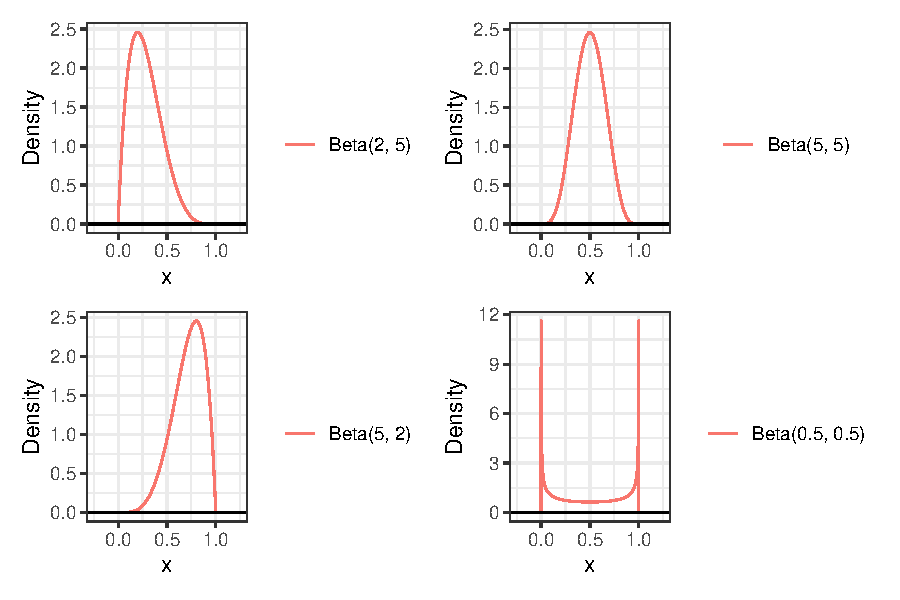
\includegraphics[width=\linewidth]{beta.plots.pdf}
\caption{Histograms for various beta distributions}
\label{fig:beta}
\end{figure}

\begin{table}[H]
\centering
\resizebox{0.4\textwidth}{!}{ 
  \begin{tabular}{rllllll}
    \hline
  & alpha & beta & mean & variance & skew & kurt \\ 
    \hline
  1 & 2.0 & 5.0 & 0.2857143 & 0.02551020 & 0.5962848 & -0.1200000 \\ 
  2 & 5.0 & 5.0 & 0.5000000 & 0.02272727 & 0.0000000 & -0.4615385 \\ 
  3 & 5.0 & 2.0 & 0.7142857 & 0.02551020 & -0.5962848 & -0.1200000 \\ 
  4 & 0.5 & 0.5 & 0.5000000 & 0.12500000 & 0.0000000 & -1.5000000 \\
    \hline
  \end{tabular}
}
\caption{Numerical summaries of beta distributions} 
\label{beta.plots:reference}
\end{table}

As you can see, I made plots for each of the four distributions using the ggplot2 \citep{ggplot} and tidyverse \citep{tidyverse} packages. The Beta(2,5) plot is skewed left, and the Beta(5,2) plot is the same graph, except skewed right. When alpha and beta are equal (5,5), the plot is symmetrical. This tells me that having a larger alpha skews the graph right, and a larger beta skews the graph left. What this means is that a larger alpha means more data will be near 1, indicating that alpha represents "successes". We can say the opposite about beta. However, you can see in the Beta(0.5,0.5) plot that it has a U-shape. This is because when the parameters are less than 1, the plot becomes bimodal with peaks near 0 and 1. This is just a result due to the probability density function of the Beta distribution. One thing to note from the table if you couldn't tell from the plots is that the mean is 0.5 if alpha and beta are equal. If alpha is larger, the mean is closer to one, and the opposite is true if beta is larger. This makes sense given the skewness we know that the parameters cause.

So now we know that if the two parameters are greater than or equal to one, the Beta distribution will have a bell-shaped curve, with its skewness dependent on which parameter is larger. If alpha is larger, it will have a right skew, and vice versa for beta. If they are equal, it will be symmetric. In the case that the parameters are less than one, the plot will take on a U-shaped curve, with peaks near zero and one. The closer the parameters are to zero, the higher the density at the ends will be. We also saw some patterns in the statistics in relation to the parameters, but we will get more into that in the next section.
\section{Properties (Mean, variance, skewness, and kurtosis)}
There are formulas with respect to alpha and beta for the mean, variance, skewness, and kurtosis of the beta distribution. Another way to caluclate these statistics is to use moments (centered and uncentered). We can then compare these results to the values we got from the original formulas to confirm that our function is working properly. In order to calcualte these statistics using moments, I used the \texttt(integrate()) function from base \texttt{R}.

One interesting thing to look at in regards to these statistics, is how their variance changes based on sample size. Is the sample skewness always going to be close to the true population skewness? If not, how big of a sample size does it take to converge? Well we can answer this question by computing the cumulative numerical summaries using the cumstats \citep{cumstats} package, while also using \texttt{geom\textunderscore line()} to plot the true population values. The patchwork \citep{patchwork} package is also useful here so that we can plot all four statistics next to each other. Lastly we will need the e1071 \citep{e1071} package so that we can use functions like \texttt{mean()}, \texttt{skewness()}, etc.

\begin{figure}[H]
  \centering
  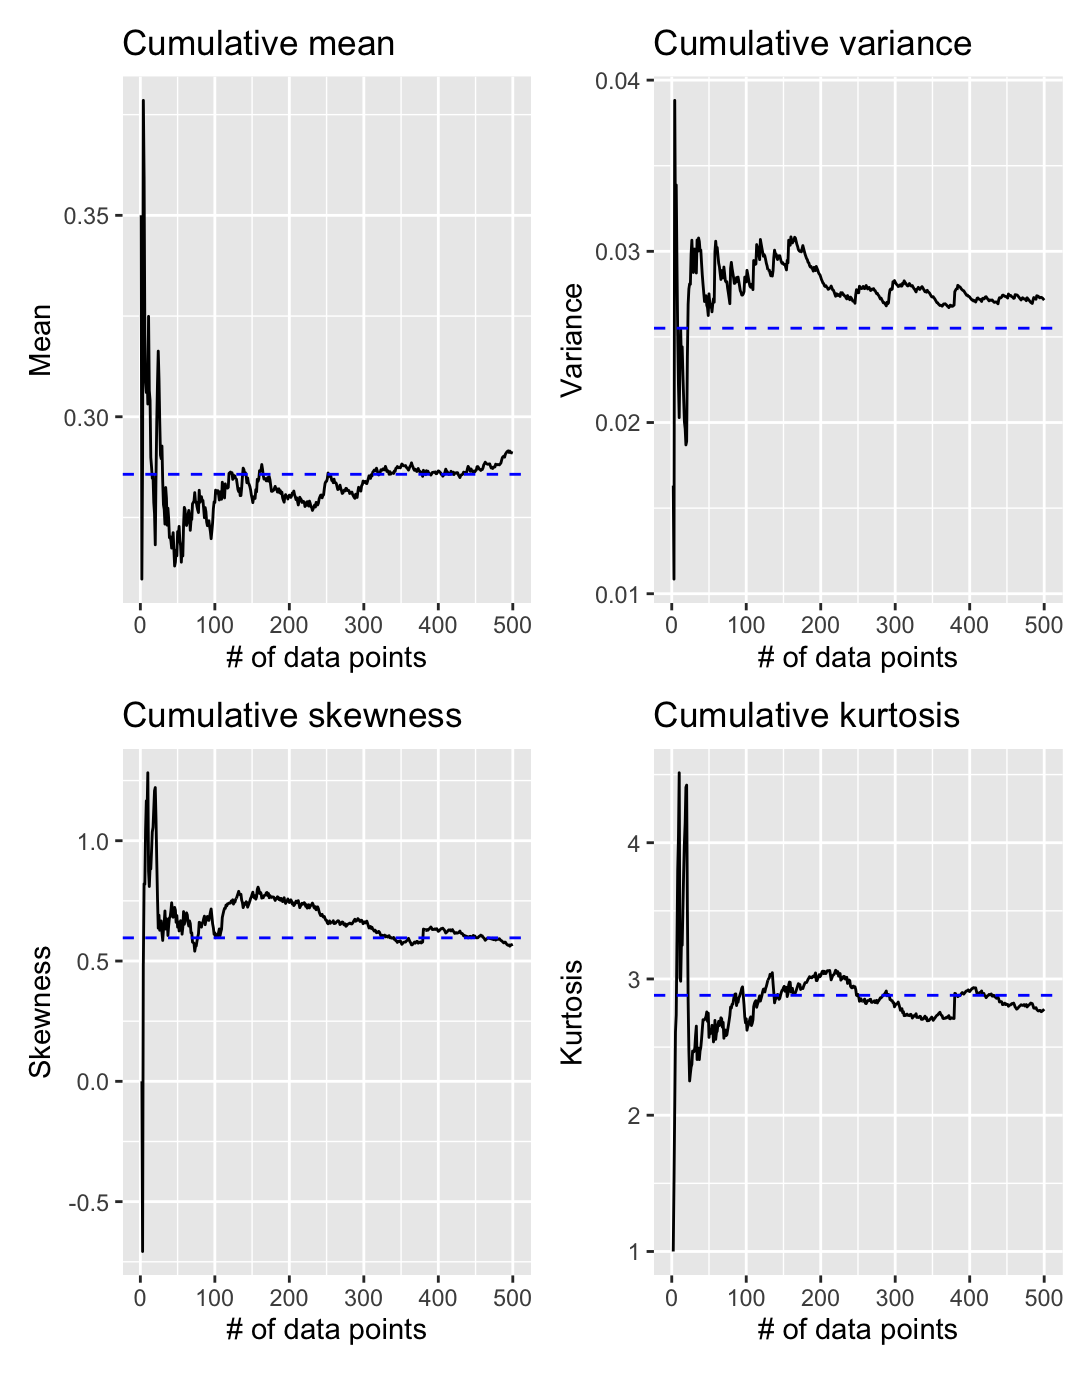
\includegraphics[width=0.6\linewidth]{cumplot.png}
  \caption{Cumulative stats for Beta(2, 5)}
  \label{fig:cumstats}
\end{figure}
As you can see in the plots, the cumulative statistics do end up converging to their true values, but it definitely takes time. For mean and kurtosis, I would say after 100 data points, the cumulative statistic stays pretty close to its true value. Variance actually stays above its true value even after 500 data points, so maybe we needed more data for variance. Skewness looks like it is converging very quickly (around 30 data points), but then goes away from its true value until around 300 data points. 

If we want to see the distribution of all of these different statistics, we can use the resampling method I mentioned earlier. I stored each statistic for 1000 different samples, and then plotted the distribution for each stat.

pdf 
  2 

\begin{figure} [H]
\centering
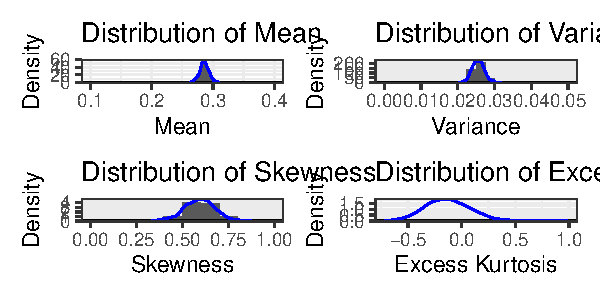
\includegraphics[width=\linewidth]{resampling.pdf}
\caption{Histograms for sampling distributions}
\label{fig:sampling}
\end{figure}

As you can see, and maybe expected, each statistic follows a relatively normal distribution.
\section{Estimators (MOM and MLE)}
The two main point estimators we work with are the Method of Moments (MOM) estimates and the Maximum Likelihood estimates (MLE). What these do is estimate the parameters of the distribution, based on the moments, or the observed data, respectively.

For MOM, we can make a function that calculates the difference between sample moments and population moments, and then use the \texttt{nleqslv()} function from the nleqslv \citep{nleqslv} package to get the best estimate for the alpha and beta parameters. For MLE, we can do the log of the PDF of the sample, and take the sum of that. Using log is easier because the log of products can be rewritten as a sum. We can then use the \texttt{optim()} function to again get the best estimate for the parameters.
I plotted a histogram of the density of my sample data, and superimposed the density lines of beta distributions with the parameters that I got from MOM and MLE. For my sample, I used data of death rates among different countries in 2022. As I said earlier, the beta distribution is good for proportions/percentages, but it is also good for any sort of rate. This is because rates are values between zero and one. To make this data usable for a beta distribution, I divided the deaths column by 1000 to convert it into a rate. After cleaning the data, I was left with a data frame with just two columns; the name of the country, and 2022 death rate. There were 263 entries after removing all missing data. 
As you can see below, the estimator lines aren't perfect, but they are pretty accurate. It's hard to tell from the plot which estimator is better in this case, so next we will try to determine that.
\begin{figure}[H]
  \centering
  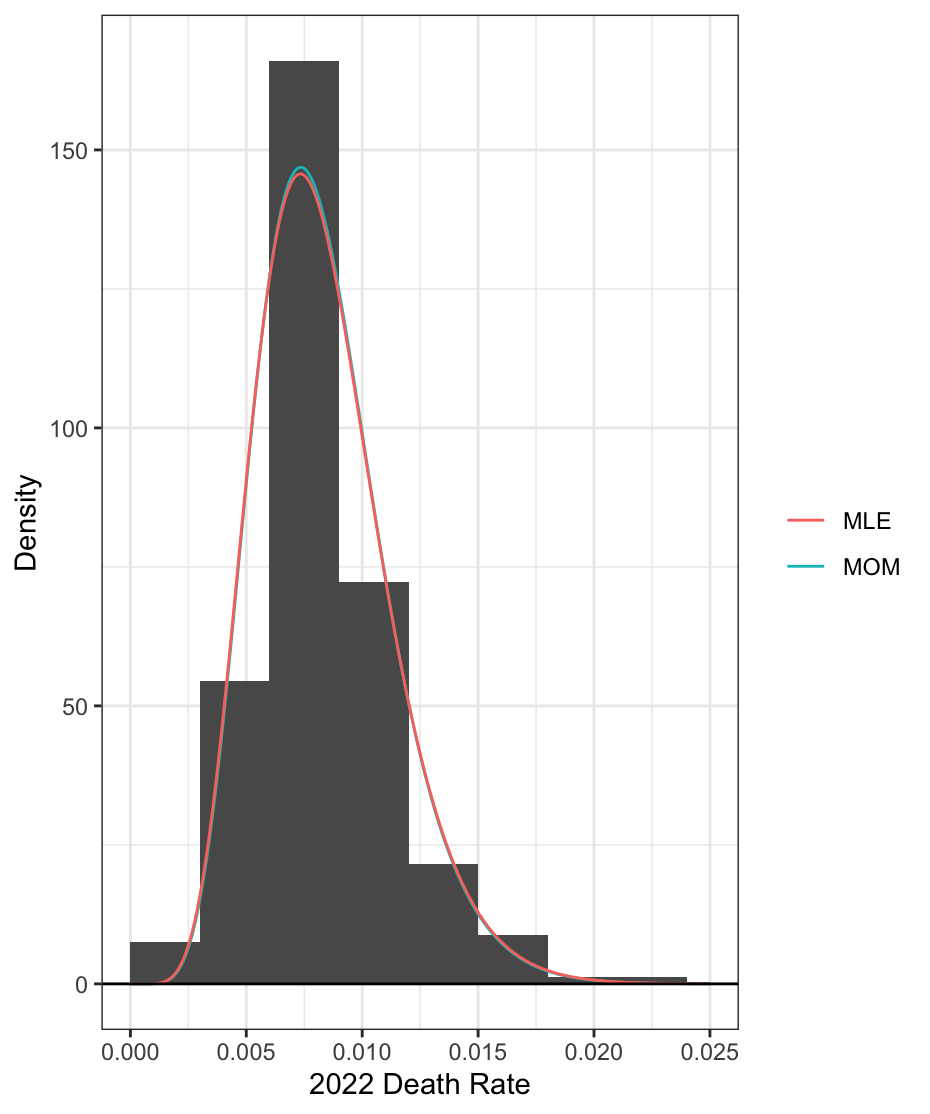
\includegraphics[width=0.7\linewidth]{estimators.png}
  \caption{Estimators for 2022 Death Rates}
  \label{fig:estimators}
\end{figure}
Now that I want to determine which estimator is more accurate, I used the resampling method again, to get the distribution of both alpha and beta, for each estimator method, giving me four distributions. It may be difficult to get the answer to the question from the plots alone, which is why I calculated the bias, precision, and mean squared error of each distribution. 
\begin{figure}[H]
  \centering
  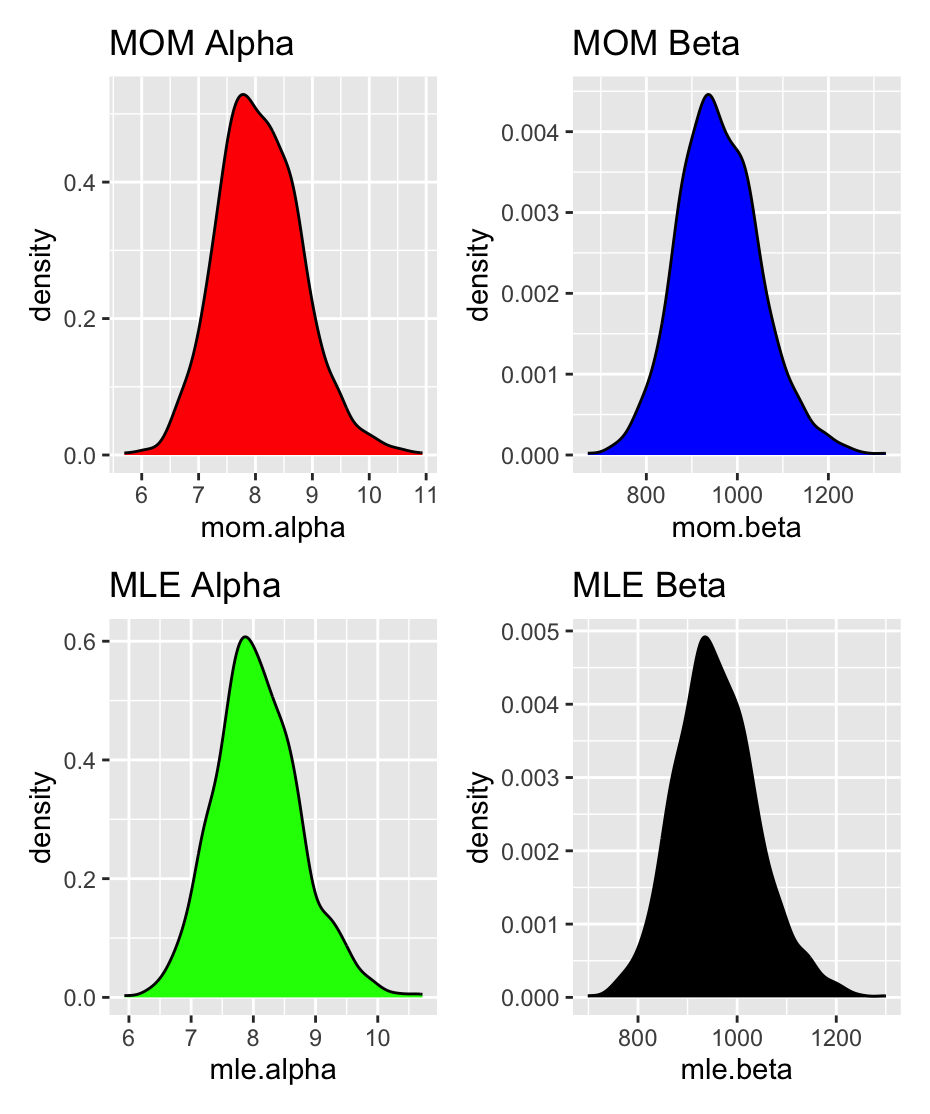
\includegraphics[width=0.7\linewidth]{bestestimator.png}
  \caption{Sampling Distributions of Estimators for 2022 Death Rates}
  \label{fig:sampling.estimators}
\end{figure}

\begin{table}[H]
\centering
\resizebox{0.4\textwidth}{!}{ 
  \begin{tabular}{rlll}
    \hline
  & Bias & Precision & MSE \\ 
    \hline
  alpha.MOM & 0.08269985 & 1.8280755792 & 0.5538626 \\ 
  beta.MOM & 10.40712130 & 0.0001221625 & 8294.1232237 \\ 
  alpha.MLE & 0.07200239 & 2.1272639221 & 0.4752718 \\ 
  beta.MLE & 9.11362689 & 0.0001418337 & 7133.5690116 \\
    \hline
  \end{tabular}
}
\caption{Numerical summaries of estimator distributions} 
\label{estimators.summary:reference}
\end{table}
As you can see in table 2, the MLE values have both a lower bias and a lower MSE than the MOM values, already making it seem like MLE is more optimal for this example. To make it more convincing, if you look at the precision column, you can see that the MLE values are more precise for both alpha and beta. I think it is safe to say that even though it's close, the MLE method is a better estimator of the beat distribution parameters for 2022 death rates.
\section{Discussion}
I have learned through this lab that using a combination of cumulative statistics, resampling, and point estimators, you can learn a lot about a probability distribution, even if there is an unknown parameter. However, without a data set that fits the basic requirements of the probability distribution, you won't be able to learn as much. We knew for the Beta distribution that we just needed continuous data ranging from 0 to 1, so pretty much any data that consists of rates will approximately fit into the Beta Distribution. The reason the Beta distribution is so easy to fit, is because of its flexibility. Alpha and Beat can take on infinitely many values, and can so drastically change the shape of the curve. Other probability distributions are probably more difficult to approximate than the Beta distribution, but I am sure that through the use of all the methods I used in this lab, you can learn a lot about any distribution.
%%%%%%%%%%%%%%%%%%%%%%%%%%%%%%%%%%%%%%%%%%%%%%%%%%%%%%%%%%%%%%%%%%%%%%%%%%%%%%%%
% Bibliography
%%%%%%%%%%%%%%%%%%%%%%%%%%%%%%%%%%%%%%%%%%%%%%%%%%%%%%%%%%%%%%%%%%%%%%%%%%%%%%%%
\vspace{2em}

\noindent\textbf{Bibliography:} 

\begin{tiny}
\bibliography{bibliography}
\end{tiny}
\end{multicols}

\end{document}
